\documentclass{article} % For LaTeX2e
\usepackage{nips13submit_e,times}
\usepackage{hyperref}
\usepackage{url}
\usepackage{graphicx}
\usepackage{amsmath}
\usepackage{amsfonts}
%\documentstyle[nips13submit_09,times,art10]{article} % For LaTeX 2.09


\title{Predicting Popularity of YouTube Video}

\author{
Loc Do \\
Heinz College,
Carnegie Mellon University \\
Pittsburgh PA, 15213\\
\texttt{halocd@andrew.cmu.edu} \\
\And
Joseph Richardson \\
School of Computer Science,
Carnegie Mellon University \\
Pittsburgh PA, 15213 \\
\texttt{jmrichar@andrew.cmu.edu} \\
}

\newcommand{\fix}{\marginpar{FIX}}
\newcommand{\new}{\marginpar{NEW}}

\nipsfinalcopy % Uncomment for camera-ready version

\begin{document}

\maketitle

\section{Introduction}
\label{sec:intro}
YouTube is one of the most popular video-sharing online platform in the Internet. It attracts billion of unique user visit monthly and has diverse topics in their video content. YouTube users can earn money from the number of views of their uploaded videos. Hence, understanding the secrets of making a popular YouTube video is essential for people who want to make benefits from the site. There are many factors to determine popularity of a video, but in general we can pin down to have the following two: having good content and good marketing plan. One of the techniques to attract more viewerships is to make the video's "visual appearance" look appealing such as catchy keywords, informative cover picture, etc. Our approach is to utilise a video's metadata to predict their popularity.

Ranking problem (aka. Learning to rank\footnote{http://en.wikipedia.org/wiki/Learning\_to\_rank}) is a typical supervised learning problem of predicting the rank of a set of items regarding to a set of criteria. It has a numerous applications in a broad domains such as web search, multimedia retrieval, recommender systems, etc. Results from these such problems can bring benefits to Internet users such as saving their time by introducing the most relevant products/articles/web pages to their interests. In YouTube context, ranking problems can be raised to recommend most relevant videos to a given video. Another application is to predict the ranking of videos w.r.t to their popularity. This can reveal the most important visual factors in determine a popularity of a video.

\textbf{Problem statement.} Given a set of videos, each is associated with a set of bag-of-word and numeric features. A pair of videos is said to have an order on their popularity by comparing their number of views. Video with more viewership is considered to be more popular than the other. Given two videos with their features, the ranking problem here is to construct a model to well predict the exact order between the two videos.

\section{Proposed solutions}
\label{sec:solution}

	\subsection{Logistic Regression on binary classification}
	We can reformulate the ranking problem between two videos as a binary classification. To be specific, let $\mathcal{X}_u \in \mathbb{R}^d$ and $\mathcal{X}_v \in \mathbb{R}^d$ represent features of video $u$ and $v$. We can form a representative vector of the two as follows

	\begin{equation}
		\mathcal{X}_{uv} = f (X_u, X_v),
	\end{equation}
	where $f: (\mathcal{R}^d, \mathcal{R}^d) \rightarrow \mathcal{R}^k$ is a transformation function. We have several options for the transformation function $f$. 
	\begin{itemize}
		\item Difference between two feature vectors: $\mathcal{X}_{uv} = X_u - X_v$
		\item Concatenation of two feature vectors:  $\mathcal{X}_{uv} = [X_u, X_v]$ (Matlab notation)
		\item Kernel functions, e.g. $\mathcal{X}_{uv} = || X_u - X_v ||^2$
	\end{itemize}
	At the moment, we cannot find any theories/signals to indicate which form of $f$ is the most appropriate. Therefore, we plan to implement all of them and compare their performance empirically. 
	
	Let define $Y_{uv}$, the label associated with the video pair $(u, v)$, as follow
		
	\begin{equation}
		Y_{uv} = \begin{cases}
				   1, & \text{if } \text{\#\_of\_view\_u} \geq \text{\#\_of\_view\_v} \\
				   0, & \text{otherwise}
				\end{cases} 
	\end{equation}
	 
	 We can assume the function form of classifier $P(Y_{uv}|\mathcal{X}_{uv})$ as follows
	 \begin{equation}
		 P(Y_{uv}=0|\mathcal{X}_{uv}) = \frac{1}{1 + \exp ( w_0 + \sum_i w_i \mathcal{X}_{uv}^i )}
	 \end{equation}
	 
	The model parameters \textbf{$w$} can be learnt efficiently using Gradient Descent algorithm. 
	
	\subsection{Linear Regression on number of views}
	Another approach to the ranking problem is to predict the number of views from a video's metadata (excluding the actual views) and use the predicted number to determine which video is more popular. This can be treated as a simple linear regression problem. Again, our linear function can be written in the functional form of feature vectors as input $X_u$ plus some noise $\epsilon$
	
	\begin{equation}
	Y_u = \beta X_u + \epsilon
	\end{equation}
	 
	 We can use the closed form or Gradient Descent to learn the $\beta$ parameters. After the learning stage, the predicted ranking can be done as follows
	 \begin{equation}
	 	\hat{Y}_{uv} = \mathbb{I}(\beta X_u > \beta X_v),\\					
	 \end{equation}
	 where $\mathbb{I}$ is the indicator function, return 1 if the expression as argument is true, and 0 otherwise.
	 
	%\subsection{First Steps Taken}
	%The data gathering required significant time, and is a big part of the project, but apart from this we had to change most of our plans regarding first steps.  Therefore, what we will present in this report is the results of our first attempt to predict the popularity of a video.  For this, we have considered the data from just five days of crawling, and we have reduced the number of fields considered to the title, uploader, video length, and upload date.  We consider only the number-predicting version, not the direct-comparison-prediction version.

	%\subsection{Technique Details}
	%We perform  a linear regression on the log of the number of views ("Y") and some features extracted from our video data ("X"), to find the best $\beta$ for $Y  = \beta * X$.  We also use the log of the number of views as our loss function, rather than using the number of views directly.

	%We then randomly select 80\% of our data for training, and reserve the other 20\% for testing.  Once the training is finished, we run the other 20\% of our data into the trained model, and consider how much loss was observed.

\section{Experimental study}
\label{sec:experiment}

	\subsection{Dataset}
	We implemented our own crawler in Java and started to collect information from YouTube since October, 1st, 2014. Our crawling strategy is to initialize the crawler with several random "seed" videos, which mostly are in the \textit{Movie} and \textit{Music} category, , and recursively explores all other videos that YouTube suggests as being related to that videos. For each video, we extract all of its metadata such as title, uploader, description, upload date, number of views/likes/dislikes, video length, and a number of other attributes, as well as a list of around 30 videos YouTube recommends as being similar. 

		\subsubsection{Preliminary Data Statistics}

		Although the crawler was suspended twice due to technical issues and upgrades, thus far we have gathered a decent amount of data:

		\begin{itemize}
			\item Number of videos crawled: 335,373
			\item Number of uploaders: 146,655
			\item Most viewed video: 2,107,560,304 views.
			\item Most "liked" video: 8,647,905 likes.
			\item Most "disliked" video: 4,184,459 dislikes.
			\item Size of "bag of words" dictionary produced for the titles: 129,553 entries.
		\end{itemize}

		As the statistics show, we have a large magnitude in ranges of number of view, likes and dislikes. This motivates us to do some preprocessing on data, such as feature normalisation or data standardization, to ensure the numerical stability and good speed of convergence on the learning algorithm. We discuss more on this step in the Section \ref{sec:preprocessing}.
		
		We plot in Figure \ref{fig:logNoOfViews} the distribution of number of views in our current data. Interestingly, the distribution is in the shape of Gaussians, instead of following the Power Law distribution as frequently observed in social network. We guess this observation is due to the way we sample the data, by following the recommended links, and imply that popularity of a video is one of the highly-impacted factors in YouTube recommender systems. Whether we can uncover the underlying reasons of links suggested by YouTube, namely, based on similarity or popularity or both, is an interesting question and may be addressed in our future work.
		
		\begin{figure}[!h]
			\begin{center}
				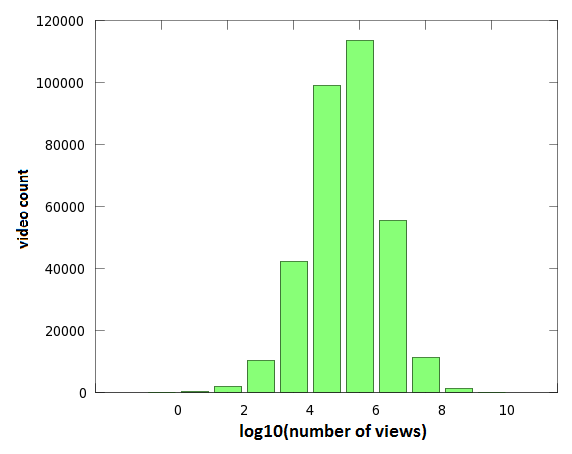
\includegraphics[width=.75\textwidth,clip]{DistributionOfViews.png}				
			\end{center}
			\caption{Histogram on the distribution of number of views (in log-scale).}
			\label{fig:logNoOfViews}
		\end{figure}
				
		\subsubsection{Pre-processing data}
		\label{sec:preprocessing}
		To Joseph: can you help me to work on this part ? You can revise from your discussion of taking the log-form and put it here.
		
		\subsubsection{Feature extraction}
		The first step is to build a dictionary mapping the uploader to the number of videos they have uploaded and the total number of views there videos have. We also take care to prevent "cheating":  In order to ensure that our predictor has only such information as would be available before the video's publishing is ever used, we temporarily reduce these number of video-views and the total number of video uploads for the uploader according to the publish date of the video under current consideration.

	We train a linear regression model for each of our three outputs on the following features:
	\begin{itemize}
		\item
		Many features extracted via a bag-of-words model on the title, using TF-IDF.
	
		\item
		The \# of videos uploaded by the uploader prior to the current video's upload date.

		\item
		The total \# of views for an uploader due to videos released prior to the current video's upload date.
		
		\item
		The fraction of the previous two features (the average number of views per video for videos uploaded by the same uploader prior to the current video's upload date).
		
		\item
		The runtime of the video, in seconds.
	
		\item
		The age of the video at the time of crawling, in days.
	\end{itemize}
	
	\subsection{Evaluation Metrics}
	Three evaluation measures widely used to evaluate ranking approaches are 0-1 loss function, Area under Curve (AUC). \textbf{0-1 loss function} is the ratio of correctly ordered video pairs over total number of pairs in testing set.
	\begin{equation}
		0/1_{loss} = \sum_{(u, v)_{test}} \frac{1}{|(u,v)_{test}|} \textbf{1}[\hat{Y}_{uv} - Y_{uv} == 0]
	\end{equation}
	Since our label values in \{0, 1\}, we use  \textbf{AUC Loss} as another ranking-based performance metric.
	\begin{equation}
		AUC_{loss} = 1 - AUC,
	\end{equation}
	where AUC is the area under the ROC curve.
%\subsection{Comparing Order-of-Magnitude}

%It is important to decide what we will consider as being "close to correct".  0-1 loss is sufficient for our comparison-based version, and for our predictors of the percentage of likes and dislikes, we can simply consider our loss in terms of the square of the difference between our prediction and the true value.  When predicting the number of views, however, we must deal with the gigantic variance in our observed data.

%Ideally, we wish to consider orders of magnitude rather than direct counts, and for this we will set our loss function equal to the square of the difference between the log of our prediction and the log of the observed value.  The motivation is that we wish to reflect the human intuition that there is more difference between the popularities of two videos with 10 and 1,000 views (respectively) than between two videos with 1,000,000 and 1,001,000.  This will prevent petty among between the most popular videos from drowning out the differences in all others.

%The decision to use a log-number-of-views-based loss function may be reversed at a later time if we find better results without it.

%Currently we are using a linear regression to predict the number of views, and we deal with the number of views in log scale for the regression.  One anticipated effect of this is that features will be expected to contribute multiplicitively, rather than additively, to the popularity of a video.  While this certainly seems interesting, it is something that we may ultimately change our minds about as we hone our results to finer detail.  As our model grows more sophisticated than mere linear regression, it may be possible to achieve multiplicitive effects when needed even while working directly with the number of views rather than its log.

	\subsection{Preliminary Results}
	Here we show some of our preliminary results using a simple linear regression.
	
\section{Related work}
\label{sec:related}

	\begin{itemize}
	\item Local Collaborative Ranking [1]
	\item Logits model for sets of ranked items [2]
	\item AdaRank [3]
	\end{itemize}

To be updated fully later with brief summary on each work

\section{Conclusion}
\label{sec:conclusion}

	\subsection{To-do list}
	There is one additional piece of information that we decided our crawler should collect, which still needs to be added: the number of subscribers for each user.  Since this was not needed for our original proposal, we will need to go back and gather this information, which may take some time considering the vast quantity of videos crawled.

	\subsection{Stretch Goals}
	We certainly hope to attempt increasingly sophisticated learning techniques to reduce our loss as much as possible.  Time allowing, there are also other interesting results we can persue.  Chief among these in our mind is to make more time-dependent predictions.  It may be, for example, that video A is very popular at first, but that video B maintains it's popularity better over time, eventually overtaking video A in terms of the numbers of views and of likes.

\subsubsection*{Acknowledgments}

Our sincere thanks to Anthony for his patience and value inputs to improve our project.

\subsubsection*{References}
\small{
[1] Joonseok Lee, Samy Bengio, Seungyeon Kim, Guy Lebanon and Yoram Singer. Local Collaborative Ranking. Proceedings of the 23rd International World Wide Web Conference (WWW) 2014

[2] Allison, Paul D., and Nicholas A. Christakis. "Logit models for sets of ranked items." Sociological methodology 24.1994 (1994): 199-228.

[3] Xu, Jun, and Hang Li. "Adarank: a boosting algorithm for information retrieval." Proceedings of the 30th annual international ACM SIGIR conference on Research and development in information retrieval. ACM, 2007.
}
\end{document}
